\begin{figure}[ht]
\centering
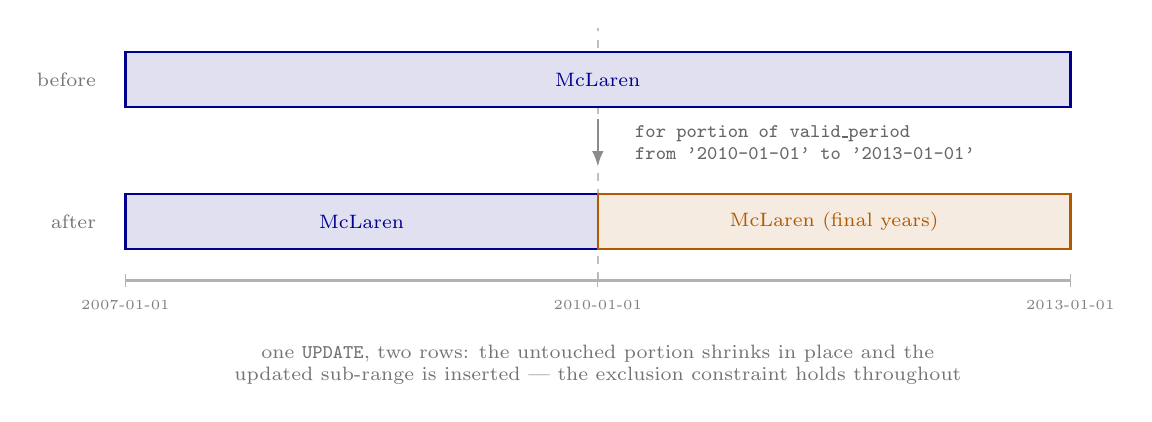
\begin{tikzpicture}[font=\small]

\colorlet{cKeep}{blue!55!black}
\colorlet{cNew}{orange!70!black}

%% Geometry: 2007 -> x=0, 2010 -> x=6, 2013 -> x=12 (2 units per year).
\def\xa{0}
\def\xb{6}
\def\xc{12}

%% The split point, carried through both rows.
\draw[black!25, dashed, line width=0.6pt] (\xb,0.55) -- (\xb,3.75);

%% ---------- before: one row, one contiguous period ----------
\node[anchor=east, font=\scriptsize, black!55] at (-0.25,3.1) {before};
\filldraw[cKeep!12, draw=cKeep, line width=0.9pt]
  (\xa,2.75) rectangle (\xc,3.45);
\node[font=\scriptsize, cKeep] at ({(\xa+\xc)/2},3.1) {McLaren};

%% ---------- the statement ----------
\draw[-latex, black!45, line width=0.9pt] (\xb,2.6) -- (\xb,2.0);
\node[anchor=west, font=\ttfamily\scriptsize, black!60, align=left]
  at (\xb+0.35,2.3) {for portion of valid\_period\\from '2010-01-01' to '2013-01-01'};

%% ---------- after: the row split in two ----------
\node[anchor=east, font=\scriptsize, black!55] at (-0.25,1.3) {after};
\filldraw[cKeep!12, draw=cKeep, line width=0.9pt]
  (\xa,0.95) rectangle (\xb,1.65);
\node[font=\scriptsize, cKeep] at ({(\xa+\xb)/2},1.3) {McLaren};

\filldraw[cNew!12, draw=cNew, line width=0.9pt]
  (\xb,0.95) rectangle (\xc,1.65);
\node[font=\scriptsize, cNew] at ({(\xb+\xc)/2},1.3) {McLaren (final years)};

%% ---------- date axis ----------
\draw[black!30, line width=0.8pt] (\xa,0.55) -- (\xc,0.55);
\foreach \x/\lbl in {0/2007-01-01, 6/2010-01-01, 12/2013-01-01} {
  \draw[black!30, thin] (\x,0.47) -- (\x,0.63);
  \node[font=\tiny, black!50, anchor=north] at (\x,0.42) {\lbl};
}

%% ---------- what changed ----------
\node[anchor=north, font=\scriptsize, black!55, align=center]
  at ({(\xa+\xc)/2},-0.15)
  {one \texttt{UPDATE}, two rows: the untouched portion shrinks in place and the\\
   updated sub-range is inserted --- the exclusion constraint holds throughout};

\end{tikzpicture}
\caption{\texttt{FOR PORTION OF} splits one row's validity period in a single statement.}
\end{figure}
